\documentclass{beamer}

% ==================================================
% Sprache & Theme (Metropolis Spruce - Herr Dayi)
% ==================================================
\usepackage[ngerman]{babel}
\usetheme[progressbar=frametitle]{metropolis}
\setbeamertemplate{frame numbering}[fraction]
\useoutertheme{metropolis}
\useinnertheme{metropolis}
\usefonttheme{metropolis}
\usecolortheme{spruce}
\setbeamercolor{background canvas}{bg=white}
\setbeamertemplate{footline}{}

% ==================================================
% Pakete
% ==================================================
\usepackage{graphicx}
\usepackage{fontspec}
\usepackage{fontawesome5}
\usepackage{qrcode}
\usepackage{amsmath, amssymb}
\usepackage{tikz}
\usepackage[most]{tcolorbox}
\usetikzlibrary{positioning, arrows.meta, shapes.geometric, calc}

% ==================================================
% Farben & Blockdesign
% ==================================================
\definecolor{primaryBlue}{RGB}{20, 50, 100}
\definecolor{accentOrange}{RGB}{220, 100, 30}
\definecolor{alertred}{HTML}{C0392B}
\definecolor{lightBlue}{RGB}{245, 248, 253}

% ==================================================
% Schriftarten & Makros
% ==================================================
\setmainfont{Noto Sans}

\newcommand{\runningMan}{%
\begin{tikzpicture}[scale=0.2, baseline=-1mm, thick]
    \draw (0,1) circle (0.4); 
    \draw (0,0.6) -- (0,-0.2); 
    \draw (0,0.4) -- (-0.6,0); 
    \draw (0,0.4) -- (0.6,0.8); 
    \draw (0,-0.2) -- (-0.5,-0.8); 
    \draw (0,-0.2) -- (0.5,0); \draw (0.5,0) -- (0.8,-0.8); 
\end{tikzpicture}}

\author{Herr \textbf{Dayi}}
\institute{Philosophie Q1}
\date{}

\begin{document}
\metroset{block=fill}

% ==================================================
% 0. Startfolie (Freud-Stil)
% ==================================================
\begin{frame}[t]{Thema: Karl Marx -- Die entfremdete Arbeit (1844)}
\centering{
  \vspace{2cm}
  {\Huge Guten Morgen \faSmile[regular] \\[0.3cm]}
  {\Large Schön, dass Ihr da seid! \\[1cm]}
  \vspace{1cm}
  {\normalsize Herr \textbf{Dayi} \\ Philosophie Q1}}
\end{frame}

% ==================================================
% 1. Einstieg: Charlie Chaplin (Moderne Zeiten, 1936)
% ==================================================
\begin{frame}[t]{\faFilm \enskip Einstieg: Charlie Chaplin -- Moderne Zeiten (1936)}
\vspace{0.4cm}

\textbf{\large \faVideo \enskip Beobachtungsauftrag:}\\[8pt]
\normalsize
Was geschieht mit Charlie an der Maschine? Wie verändern sich Körper, Geist und Verhalten?\\[1.2cm]

\Large \textbf{\faExclamationTriangle \enskip Problem / Leitfrage:}

% Maximaler Freiraum zum Mitschreiben an der Tafel / am Smartboard
\vfill

\end{frame}

% ==================================================
% Agenda: Heutiger Plan (nach der Problemerarbeitung)
% ==================================================
\setbeamercovered{transparent}
\begin{frame}[t]{\faListUl \enskip Heutiger Plan}
\vspace*{0.35cm}
\begin{itemize}
    \setlength{\itemsep}{12pt}
    
    \item<1->[1.] \textbf{\large \faQuoteLeft \enskip Erschließung: Die Kernaussagen}
    
    \item<2->[2.] \textbf{\large \faSlidersH \enskip Rekonstruktion: Kernaussagen-Board am Beamer}
    
    \item<3->[3.] \textbf{\large \faProjectDiagram \enskip Erarbeitung \& Sicherung: Die 4 Dimensionen der Entfremdung}
    
    \item<4->[4.] \textbf{\large \faImages \enskip Transfer: Marx im Meme}
    
    \item<5->[5.] \textbf{\large \faCheckCircle \enskip Check-Out}
    
\end{itemize}
\setbeamercovered{invisible}
\end{frame}

% ==================================================
% 1. Erschließung: Kernaussagen (Think & Group)
% ==================================================
\begin{frame}[t]{\faQuoteLeft \enskip 1. Erschließung: Die Kernaussagen}
\vspace{0.2cm}

\begin{itemize}
    \item[] \textbf{\faStream \enskip Textausschnitte:} \newline
    \normalsize Jede Gruppe erhält \textbf{einen isolierten Satz} aus einem philosophischen Text.
\end{itemize}

\vspace{0.3cm}

\begin{itemize}
    \item[] \textbf{\faPen \enskip Arbeitsaufträge in der Gruppe:}
    \vspace{0.15cm}
    \begin{itemize}\normalsize
        \item[\textbf{1.}] \textbf{Eigene Worte:} Was will uns der Philosoph mit diesem Satz sagen? Formuliert eine prägnante Erklärung.
        \vspace{0.15cm}
        \item[\textbf{2.}] \textbf{Chaplin-Bezug \& Alltag:} Passt dieser Satz zu Chaplins Fabrikschicksal? Findet ein heutiges Beispiel.
    \end{itemize}
\end{itemize}

\vspace{0.5cm}
\begin{itemize}
    \item[] \textbf{\faUsers \enskip Sozialform:} Kleingruppen \quad \textbf{\faClock \enskip Zeit:} ca. 8--10 Min.
\end{itemize}

\end{frame}

% ==================================================
% 2. Rekonstruktion: Kernaussagen-Board am Beamer
% ==================================================
\begin{frame}[t]{\faSlidersH \enskip 2. Rekonstruktion: Kernaussagen-Board}
\vspace{0.1cm}

\textbf{\faSlidersH \enskip Arbeitsauftrag:}\\[2pt]
\small Bringt die 4 Aussagen am Beamer in eine \textbf{logische Reihenfolge} (Ursache $\rightarrow$ Folge) und begründet eure Kurshypothese!\\[8pt]

\begin{columns}[T]
    \begin{column}{0.68\textwidth}
        \centering
        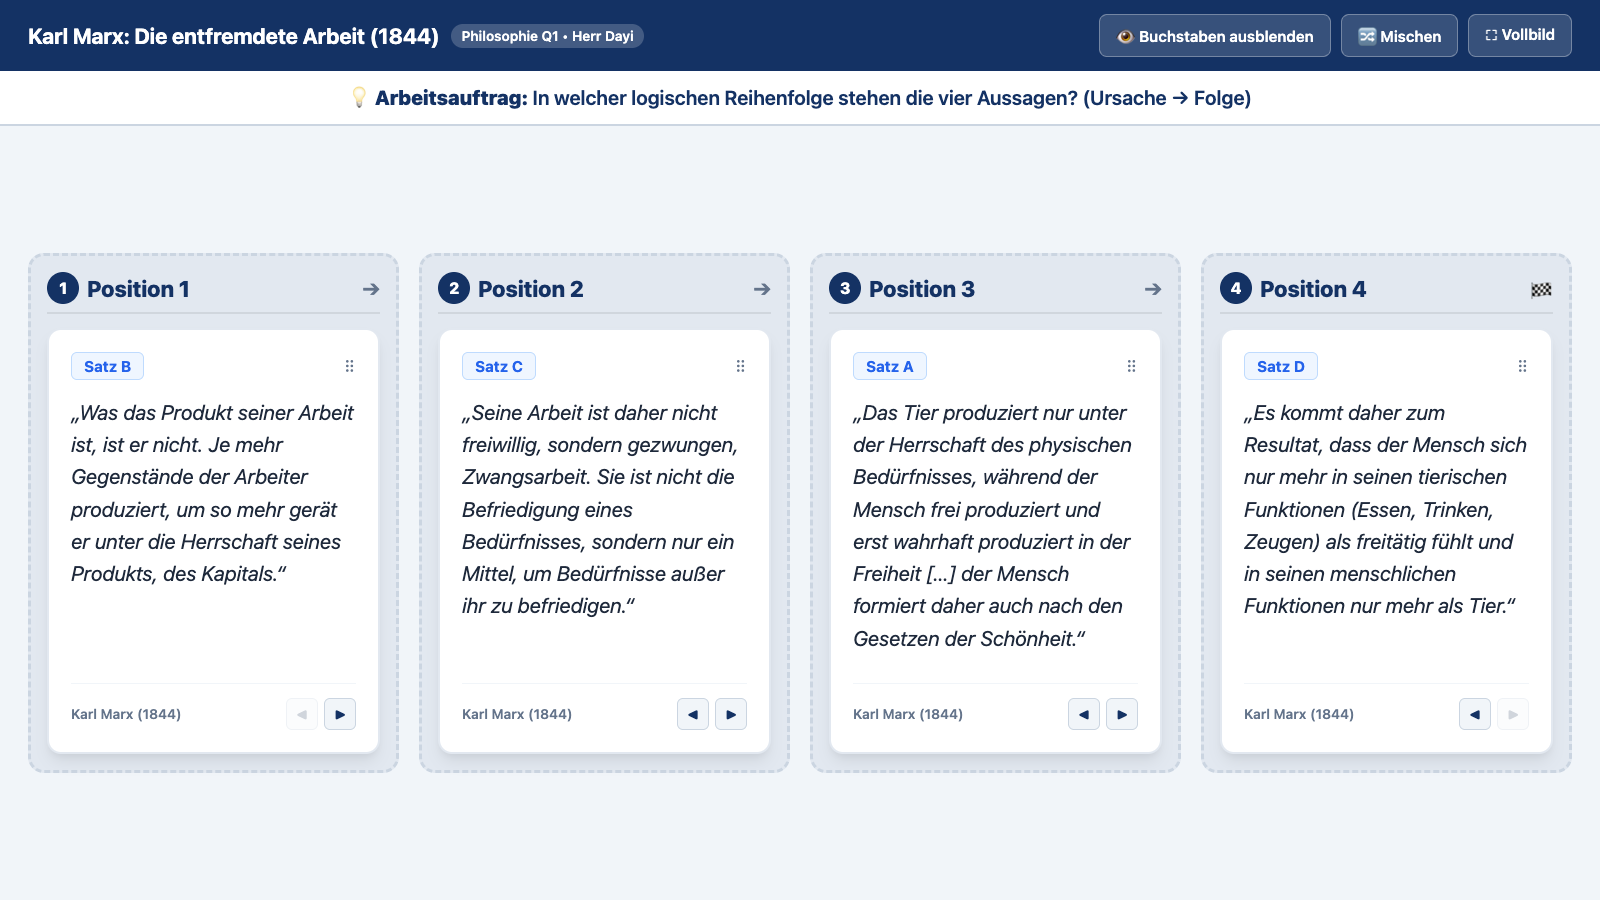
\includegraphics[width=\linewidth, height=0.58\textheight, keepaspectratio]{screenshot_board.png}
    \end{column}
    \begin{column}{0.30\textwidth}
        \centering
        \vspace{0.3cm}
        \qrcode[height=1.8cm]{https://herrdayi.github.io/Anordnung/}\\[4pt]
        {\scriptsize\textbf{\color{primaryBlue}Anordnungs-Board}}\\[2pt]
        {\tiny \href{https://herrdayi.github.io/Anordnung/}{herrdayi.github.io/Anordnung}}
    \end{column}
\end{columns}

\end{frame}

% ==================================================
% 3. Erarbeitung: Schulbuchtext (S. 168–170)
% ==================================================
\begin{frame}[t]{\faBookOpen \enskip 3. Erarbeitung: Schulbuchtext (S. 168--170)}
\vspace{0.1cm}

\begin{columns}[T]
  \begin{column}{0.72\textwidth}
    \textbf{\faPen \enskip Arbeitsauftrag:}\\[4pt]
    \begin{itemize}\small
        \item[\textbf{1.}] \textbf{Textabgleich:} Findet eure Kernaussage im Text wieder und markiert sie. Hatten wir am Beamer recht?
        \vspace{0.1cm}
        \item[\textbf{2.}] \textbf{Entfremdungsdimension:} Welcher Aspekt der Entfremdung wird in eurem Textabschnitt beschrieben?
    \end{itemize}
    \vspace{0.3cm}
    \begin{itemize}\small
        \item[\faUsers] \textbf{Sozialform:} PA / Kleingruppe \quad \textbf{\faClock} \textbf{Zeit:} ca. 20 Min.
    \end{itemize}
  \end{column}

  \begin{column}{0.26\textwidth}
    \begin{center}
      \qrcode[height=1.8cm]{https://herrdayi.github.io/Marx/}\\[4pt]
      {\scriptsize\textbf{Hilfestellung}}\\[1pt]
      {\tiny (Glossar \& Tipps)}
    \end{center}
  \end{column}
\end{columns}

\vspace{0.3cm}
\footnotesize
\begin{itemize}
   \item[] \runningMan \, \textbf{Sprinter-Aufgabe:} \newline
   Vergleicht Marx mit Rousseau: Wo verortet Marx das \glqq wahre Wesen\grqq{} des Menschen -- im Urzustand oder im bewussten Arbeiten?
\end{itemize}

\end{frame}

% ==================================================
% Sicherung: Die 4 Dimensionen der Entfremdung (LEER für Tafelbild)
% ==================================================
\begin{frame}[t]{\faProjectDiagram \enskip Sicherung: Die 4 Dimensionen der Entfremdung}

% Maximaler Freiraum für die gemeinsamen Schülerergebnisse (Tafelbild / Smartboard)
\vfill

\end{frame}

% ==================================================
% 4. Transfer: Marx im Meme
% ==================================================
\begin{frame}[t]{\faImages \enskip 4. Transfer: Marx im Meme}
\vspace{-0.1cm}

\textbf{\large \faLightbulb \enskip Arbeitsauftrag:}\\[4pt]
\normalsize
Stellt Karl Marx’ Kritik der entfremdeten Arbeit in einem \textbf{pointierten Meme} dar!
\vspace{0.25cm}

\begin{columns}[T]
    \begin{column}{0.56\textwidth}
        \textbf{\small \faPalette \enskip Freie Formatwahl:}\\[6pt]
        \small
        \begin{itemize}
            \setlength{\itemsep}{8pt}
            \item[\faLaptopCode] \textbf{Digital:} Freie Vorlage im Meme-Generator wählen und eigenen Text setzen.
            \item[\faPen] \textbf{Analog:} Die 4-Panel Comic-Vorlage nutzen (freie Skizzen, Dialoge \& Pointen).
        \end{itemize}
    \end{column}
    
    \begin{column}{0.42\textwidth}
        \centering
        \textbf{\small \faQrcode \enskip Meme-Generator}\\[5pt]
        \qrcode[height=1.9cm]{https://imageresizer.com/de/meme-generator}\\[4pt]
        {\scriptsize \href{https://imageresizer.com/de/meme-generator}{\textbf{\color{primaryBlue}imageresizer.com}}}\\[2pt]
        {\tiny \color{gray}(Kostenlos \& ohne Anmeldung)}
    \end{column}
\end{columns}

\vspace{0.4cm}
\centering
{\small \textbf{\faUsers \enskip Sozialform:} EA / PA \qquad \textbf{\faClock \enskip Zeit:} ca. 15 Min.}

\end{frame}

% ==================================================
% 5. Check-Out (Freud-Stil)
% ==================================================
\begin{frame}[t]{\faCheckCircle \enskip 5. Check-Out}
\vspace{0.5cm}

\begin{itemize}
    \setlength{\itemsep}{1.2cm}
    \item[\Large\faLightbulb] \Large \textbf{1. Ich weiß jetzt \dots}
    \item[\Large\faBrain] \Large \textbf{2. Besonders spannend fand ich heute \dots}
    \item[\Large\faQuestionCircle] \Large \textbf{3. Diese Frage nehme ich mit \dots}
\end{itemize}
\end{frame}

\end{document}
